% mn2esample.tex
%
% v2.1 released 22nd May 2002 (G. Hutton)
%
% The mnsample.tex file has been amended to highlight
% the proper use of LaTeX2e code with the class file
% and using natbib cross-referencing. These changes
% do not reflect the original paper by A. V. Raveendran.
%
% Previous versions of this sample document were
% compatible with the LaTeX 2.09 style file mn.sty
% v1.2 released 5th September 1994 (M. Reed)
% v1.1 released 18th July 1994
% v1.0 released 28th January 1994

\documentclass[useAMS,usenatbib]{mn2e}
\usepackage{graphicx,subfigure}
\usepackage{amsmath}
\usepackage{rotating}
\usepackage{color}
\usepackage{times}

%\author[dd]{dd}
\begin{document}
\def \apj {ApJ}
\def \apss {Ap{\&}SS}
\def \mnras {MNRAS}
\def \aj {AJ}
\def \araa {ARA\&A}
\def \aapr {A\&ARv}
\def \pasa {PASA}
\def \aap {AAP}
\def \aaps {AAPS}
\def \apjl {ApJL}
\def \apjs {ApJS}
\def \pasj {PASJ}
\def \nat {Nature}
% remove the useAMS option.
%
% useAMS allows you to obtain upright Greek characters.
% e.g. \umu, \upi etc.  See the section on "Upright Greek characters" in
% this guide for further information.
%
% If you are using AMS 2.0 fonts, bold math letters/symbols are available
% at a larger range of sizes for NFSS release 1 and 2 (using \boldmath or
% preferably \bmath).
%
% The usenatbib command allows the use of Patrick Daly's natbib.sty for
% cross-referencing.
%
% If you wish to typeset the paper in Times font (if you do not have the
% PostScript Type 1 Computer Modern fonts you will need to do this to get
% smoother fonts in a PDF file) then uncomment the next line
% \usepackage{Times}

%%%%% AUTHORS - PLACE YOUR OWN MACROS HERE %%%%%

\newcommand{\kpc}{{\rm\,kpc}}
\newcommand{\mpc}{{\rm\,Mpc}}
\newcommand{\pc}{{\rm\,pc}}
\newcommand{\kms}{{\rm\,km\,s^{-1} }}
\newcommand{\msun}{{\rm\,M_\odot }}
\newcommand{\lsun}{{\rm\,L_\odot }}
\newcommand{\rsun}{{\rm\,R_\odot}}
\newcommand{\ngcs}{NGC~147 }
\newcommand{\ngcf}{NGC~185 }
%\newcommand{\deg}{^\circ}

\newcommand{\km}{{\rm\,km}}
\newcommand{\cm}{{\rm\,cm}}
\newcommand{\yr}{{\rm\,yr}}
\newcommand{\au}{{\rm\,AU}}
\newcommand{\g}{{\rm\,g}}
%***************\newcommand{\om}{\Omega_0}
%***************\newcommand{ \ca} {{\it ca.\/}}
%***************%\newcommand{ \r} {r$^{1/4}$ }
%***************\newcommand{ \magnitude} {$^{\rm m}$}
%***************\newcommand{\kr}{${\cal K}_r$}
%***************\newcommand{\kz}{${\cal K}_z$}
%***************\newcommand{\kzz}{${\cal K}_z(z)$}
%***************\newcommand{\mss}{{\rm M}_\odot \rm pc^{-2}}
%***************\newcommand{\msss}{{\rm M}_\odot \rm pc^{-3}}
%***************\newcommand{\fmmm}[1]{\mbox{$#1$}}
%***************\newcommand{\scnd}{\mbox{\fmmm{''}\hskip-0.3em .}}
%***************\newcommand{\scnp}{\mbox{\fmmm{''}}}
%***************\newcommand{\mcnd}{\mbox{\fmmm{'}\hskip-0.3em .}}
\newcommand{\Aa}{\; \buildrel \circ \over {\rm A}}
%***************%\newcommand{\AA}{$\; \buildrel \circ \over {\rm A}$}
%***************
%***************% MISCELLANEOUS:
%***************% angles in degrees
%***************%\degg produces degree symbol so that 3\sec5 produces 3.`5 with the degree
%***************%symbol and the period aligned.
%***************\newcommand{\degg}{\hbox{$\null^\circ$\hskip-3pt .}}
%***************%\sec produces arcsec symbol so that 3\sec5 produces 3."5 with the second
%***************%symbol and the period aligned.
%***************%\newcommand{\sec}{\hbox{"\hskip-3pt .}}
%***************\newcommand{\half}{{\scriptstyle{1\over2}}}
%***************%\s produces tilde in mathmode or horizontal mode.
%***************\newcommand{\s}{\ifmmode \widetilde \else \~\fi}
%***************%\newcommand{\=}{\overline}
%***************\newcommand{\scre}{{\cal E}}
%***************%\newcommand{\spose#1{\hbox to 0pt{#1\hss}}
%***************\newcommand{\larrow}{\leftarrow}
%***************\newcommand{\rarrow}{\rightarrow}
%***************\newcommand{\llangle}{\langle\langle}
%***************\newcommand{\rrangle}{\rangle\rangle}
%***************\newcommand{\etal}{{\it et al.\ }}
%***************\newcommand{\cf}{{\it cf.\ }}
%***************\newcommand{\eg}{{e.g.,\ }}
%***************\newcommand{\ie}{{i.e.,\ }}
%***************%\lta and \gta produce > and < signs with twiddle underneath
%***************\newcommand{\lta}{\mathrel{\spose{\lower 3pt\hbox{$\mathchar"218$}}
%***************     \raise 2.0pt\hbox{$\mathchar"13C$}}}
%***************\newcommand{\gta}{\mathrel{\spose{\lower 3pt\hbox{$\mathchar"218$}}
%***************     \raise 2.0pt\hbox{$\mathchar"13E$}}}
%***************%\Dt and \dt put Newton's notation dots above upper and lower case chars
%***************\newcommand{\Dt}{\spose{\raise 1.5ex\hbox{\hskip3pt$\mathchar"201$}}}    % upper case
%***************\newcommand{\dt}{\spose{\raise 1.0ex\hbox{\hskip2pt$\mathchar"201$}}}    % lower case
%***************\newcommand{\del}{\nabla}
%***************\newcommand{\delv}{\bb\nabla}
%***************%\newcommand{\r}{${\rm r^{1/4}}$}
%***************
%***************\newcommand{\jla}{J_{\lambda}}
%***************\newcommand{\jmu}{J_{\mu}}
%***************\newcommand{\jnu}{J_{\nu}}
%***************\newcommand{\pomega}{\varpi}
%***************\newcommand{\sigla}{\sigma_{\lambda}}
%***************\newcommand{\sigmu}{\sigma_{\mu}}
%***************\newcommand{\signu}{\sigma_{\nu}}
%***************\newcommand{\dotsfill}{\leaders\hbox to 1em{\hss.\hss}\hfill}
%***************%\newcommand{\sun}{\odot}
%***************%\newcommand{\earth}{\oplus}
%***************
%***************\newcommand{\Gyr}{{\rm\,Gyr}}
%***************\newcommand{\FeH}{{\rm[Fe/H]}}
%***************\newcommand{\kmsd}{{\rm\,km/s/degree}}
%***************
%***************\newcommand{\ud}{\mathrm{d}}
%***************
%***************\newcommand{\ngcs}{NGC~147}
%***************\newcommand{\ngcf}{NGC~185}
%***************
%%%%%%%%%%%%%%%%%%%%%%%%%%%%%%%%%%%%%%%%%%%%%%%%

\title[Planes in Illustris and Elvis]{Planes in Illustris and Elvis}
\author[Arias et al.]{
{\parbox{\textwidth}{
Veronica Arias$^{1}$\thanks{E-mail:v.arias@uniandes.edu.co}, 
Jaime Forero$^1$,
%Nicholas F. Bate$^$,
%Anthony Conn$^2$,
%Rodrigo A. Ibata$^3$,
%Nuwanthika Fernando$^2$, 
%Alan W. McConnachie$^3$, 
%Nicolas Martin$^{5,6}$, 
et~al.\\}}
\vspace{0.1cm}\\
\parbox{\textwidth}{
$^1$Departamento de F\'isica, Universidad de los Andes, Cra. 1 No. 18A-10, Edificio Ip, Bogot\'a, Colombia\\
%$^3$Observatoire de Strasbourg, 11, rue de l'Universit\'e, F-67000, Strasbourg, France\\
%$^4$NRC Herzberg Institute for Astrophysics, 5071 West Saanich Road, Victoria, British Columbia, Canada, V9E 2E7 \\
%$^5$Institute for Astronomy, University of Edinburgh, Royal Observatory, Blackford Hill, Edinburgh, EH9 3HJ, U.K. \\
%$^6$Max-Planck-Institut für Astronomie, Königstuhl 17, D-69117 Heidelberg, Germany\\
}}

\date{Accepted xxx. Received xxxx; in original form xxxx}

\pagerange{\pageref{firstpage}--\pageref{lastpage}} \pubyear{2002}

\maketitle

\label{firstpage}

\begin{abstract}

\end{abstract}

\begin{keywords}
%galaxies -- XXX -- XXX 
Local Group --- galaxies: dwarf -- galaxies: individual (M31)  
\end{keywords}

\section{Introduction}

Observational evidence of planes is everywhere (where we can see them). MW, M31, Centaurus A.\\

Not so evident in simulations:\\

Millenium II Baumgardt, Ibata, Pawlowski\\

Clues Gillet está pero diferente\\

Plane claims:\\
Libeskind: preferential direction for accretion.\\
Sawala: planes are there when baryonic physics is included.\\
Buck: planes are easy to form at early times, when DM filaments are very thin. In high redshift galaxies galaxies, planes are everywhere.\\

Other explanations: Kroupa: tidal dwarfs\\
Fouquet\\



 
Following a bit on the claim by Sawala that barionic physics are important when looking for planes, WE look in Illustris and Elvis simulations to try and understand why barionic physics results in planar distribution of satellites.


\section{Method}
\label{Method}


\section{Results}
\label{Results}
\begin{figure}
\centering
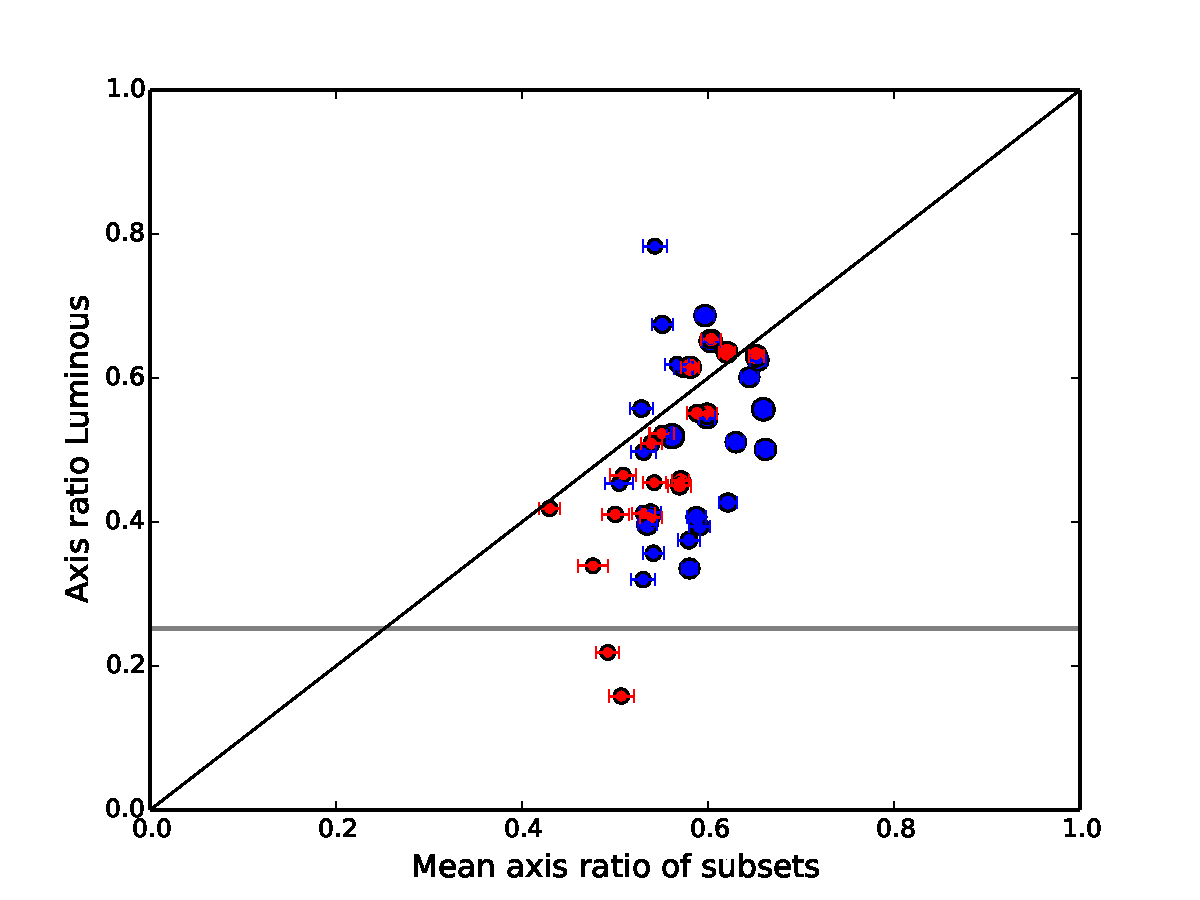
\includegraphics[width=\hsize]{AxisRatio_RandomMean_VS_Luminous.pdf}\\
\caption{.}
\label{fig:StreamPlaneOrbit}
\end{figure}

%\begin{figure}
%\centering
%\includegraphics[width=\hsize]{Halo_pos_LRomulusRemus.pdf}\\
%\end{figure}

\section{Discussion} 
\section{Acknowledgements}
%M. G. acknowledges the Australia Postgraduate Award (APA) for supporting her PhD candidature and the Astronomical Society of Australia for its travel support. 
%N. F. acknowledges the Dean's International Post Graduate Scholarship of the Faculty of Science, University of Sydney.
\bibliographystyle{mn2e}
\bibliography{Dwarfs}



\label{lastpage}

\end{document}
